%! TeX program = lualatex
% use lualatex as primary compiler
\documentclass{beamer}

% Selects the theme defined in `beamerthemeUW.sty`
\usetheme{UW}

\usepackage{packages}
\usepackage{macros}
\usepackage{tcolorbox}
\usepackage{adjustbox}
\usepackage{graphicx}


\title[RSLDS]{\small Bayesian Learning and Inference \\ in Recurrent Switching Linear Dynamical Systems}
%\subtitle{Subtitle}
%\author{Jane Doe\inst{1} \and John Doe\inst{2}}
\author{Charbel Abi Younes, Marvyn Bailly, Bart Boom, Rohin Gilman, Daran Xu}
\department{Applied Mathematics}
%\institute{
%    \inst{1}Very Fancy University \\
%    \inst{2}Another Fancy University
%}


\begin{document}

% The title slide
\begin{frame}
    \maketitle
\end{frame}

% The TOC
\begin{frame}{Table of Contents}
    \setcounter{framenumber}{1} % Sets the TOC to be the first numbered frame
    \tableofcontents
\end{frame}

\section{Introduction and Motivation}

\begin{frame}{Frame Title}{Frame Subtitle}
        Rohin

    \end{frame}

\section{Model}

\begin{frame}{Model}{SLDS and rSLDS}

\begin{tcolorbox}[colback=blue!10!white,colframe=blue!50!black,title=Model Set-up,boxrule=2pt, boxsep=0.1em, left=0.1em, right=0.1em,
fontupper=\fontsize{8}{10}\selectfont] %,height=2in
\begin{enumerate}[\textbullet]
\item Observation $y_t=C x_t+d+w_t\text{, }w_t \overset{\mathrm{iid}}{\sim} \mathcal{N}(0,S)$
\item Continous latent state $x_{t+1}=A_{z_{t+1}}x_t+b_{z_{t+1}}+\nu_t \text{, } \nu_t \overset{\mathrm{iid}}{\sim} \mathcal{N}(0,Q_{z_{t+1}})$
    \item Discrete latent state $z_t \in \{1,\dots,K\}$
        \begin{itemize}
            \item SLDS 
$z_{t+1} | z_t \sim \pi_{z_t}$
            \item rSLDS
 $z_{t+1} | z_t, x_t \sim \pi_{SB}(v_{t+1})$, $v_{t+1}=R_{z_t}x_t+r_{z_t}$
        \end{itemize}
\end{enumerate}
\end{tcolorbox}

\begin{figure}
    \centering
    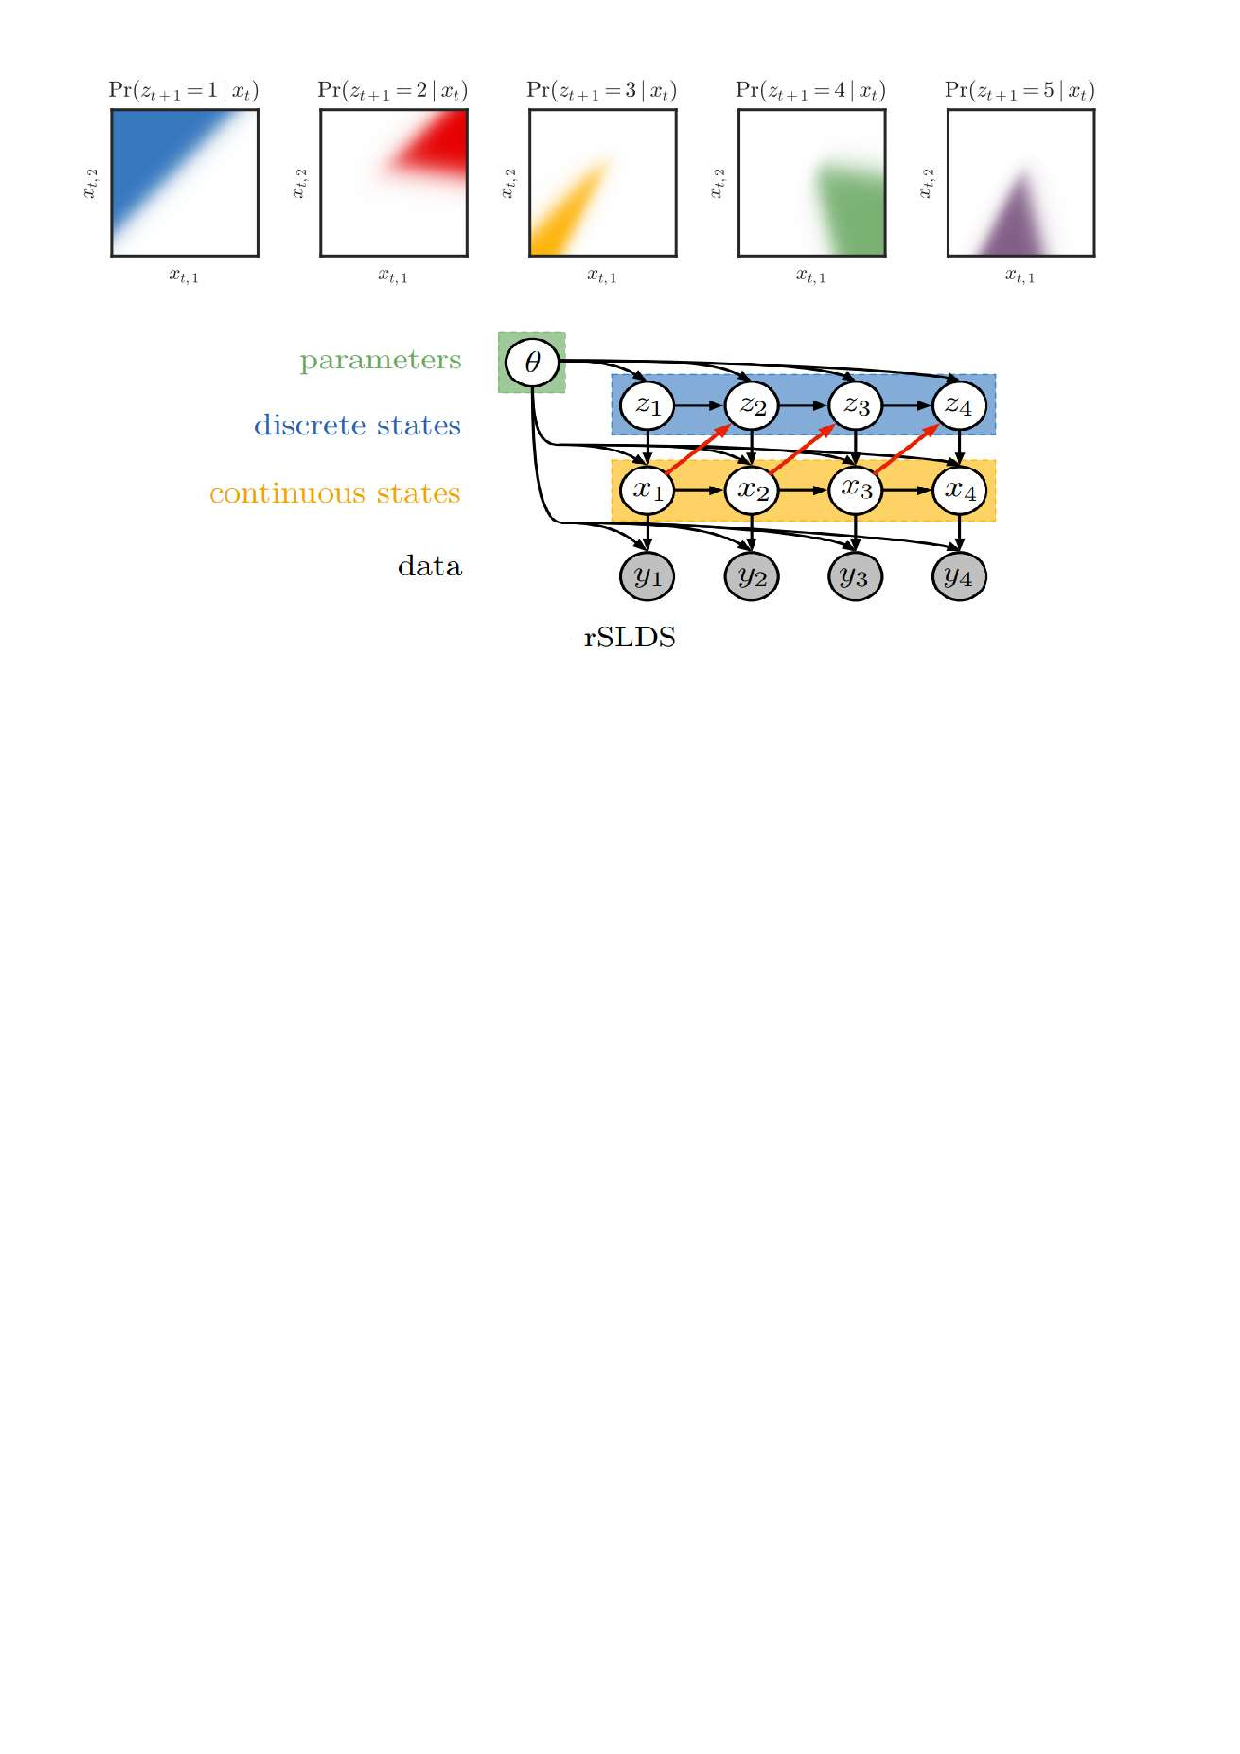
\includegraphics[width=0.7\linewidth]{gallery/model_p1.pdf}
    \caption{}
  \end{figure}



%\begin{figure}
%    \centering
%    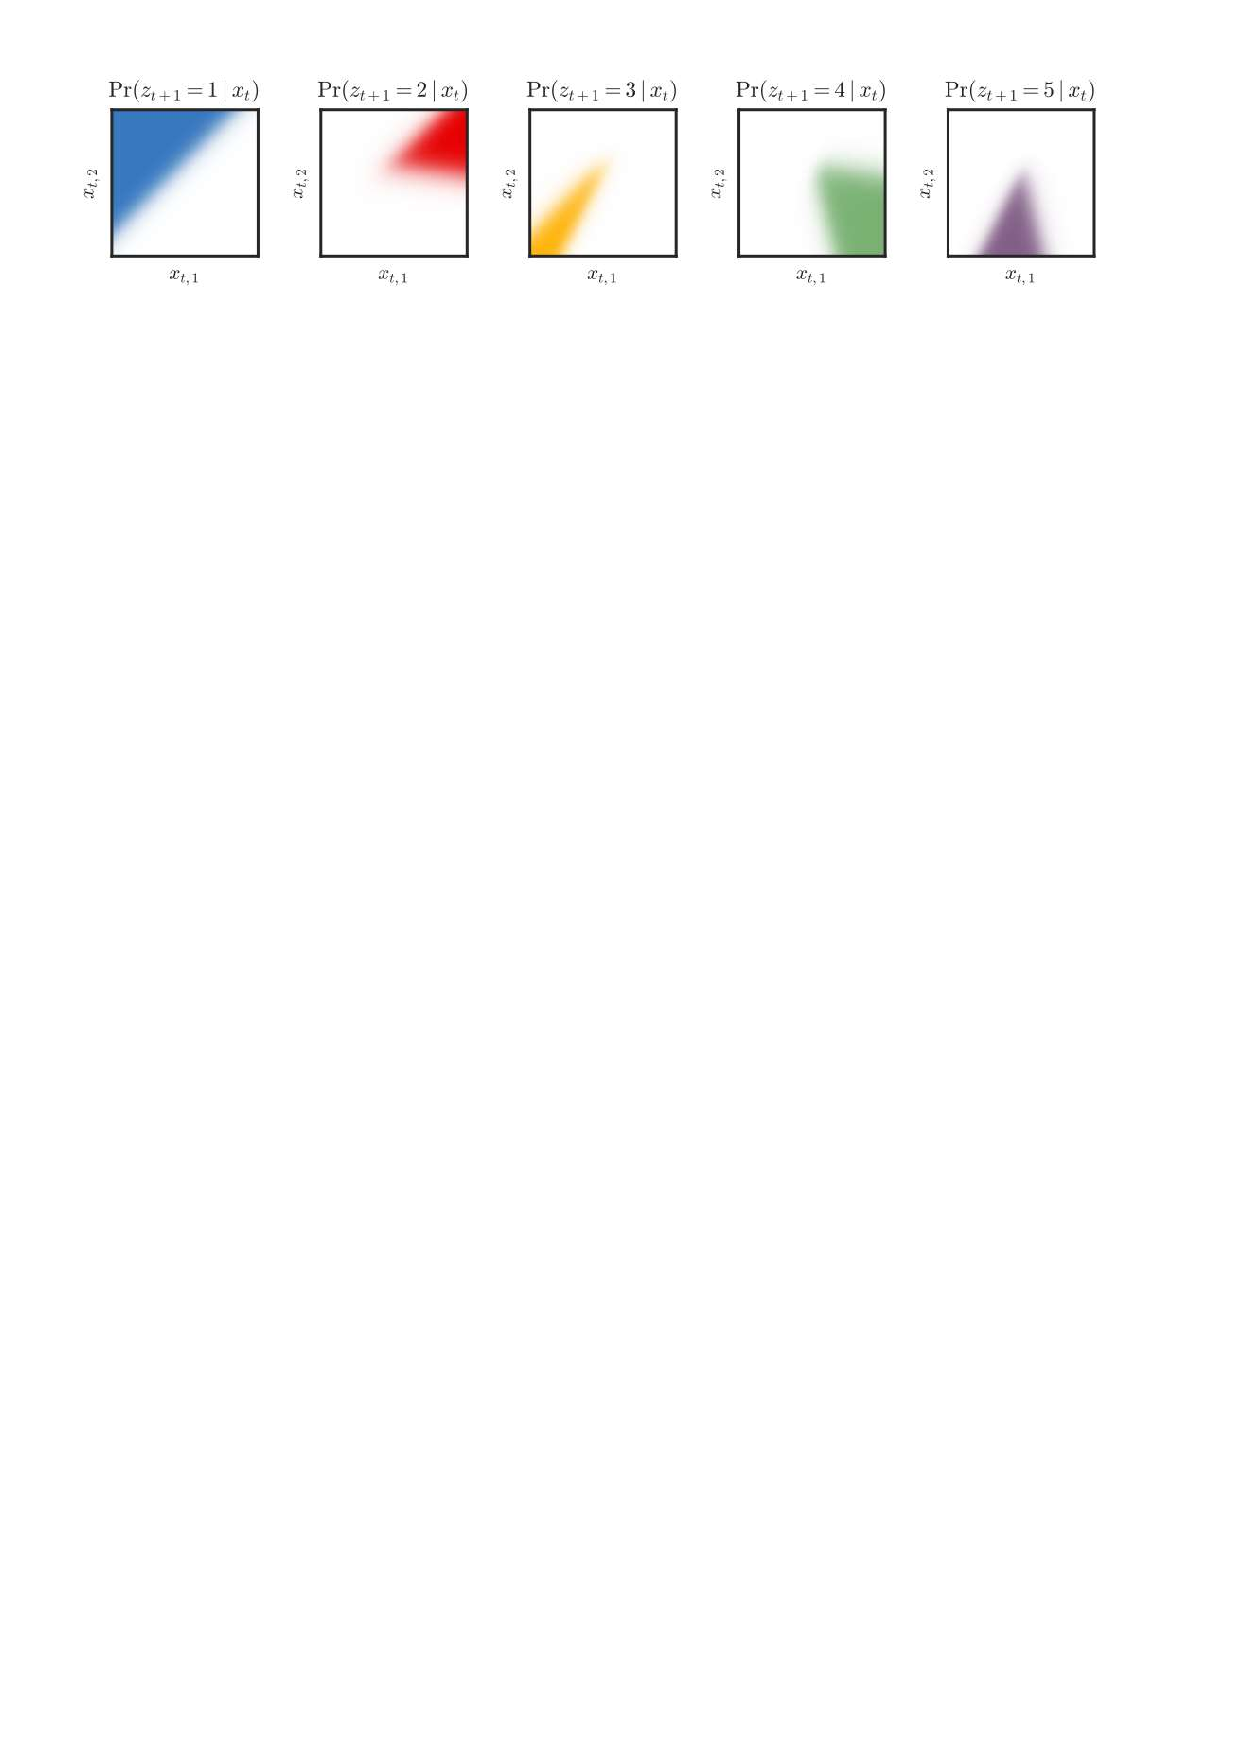
\includegraphics[scale=0.3]{gallery/z_on_x.pdf}
%    \caption{Dependence of $z_{t+1}$ on $x_t$}
%    \label{rLSDS}
%\end{figure}
%\begin{figure}
%    \centering
%    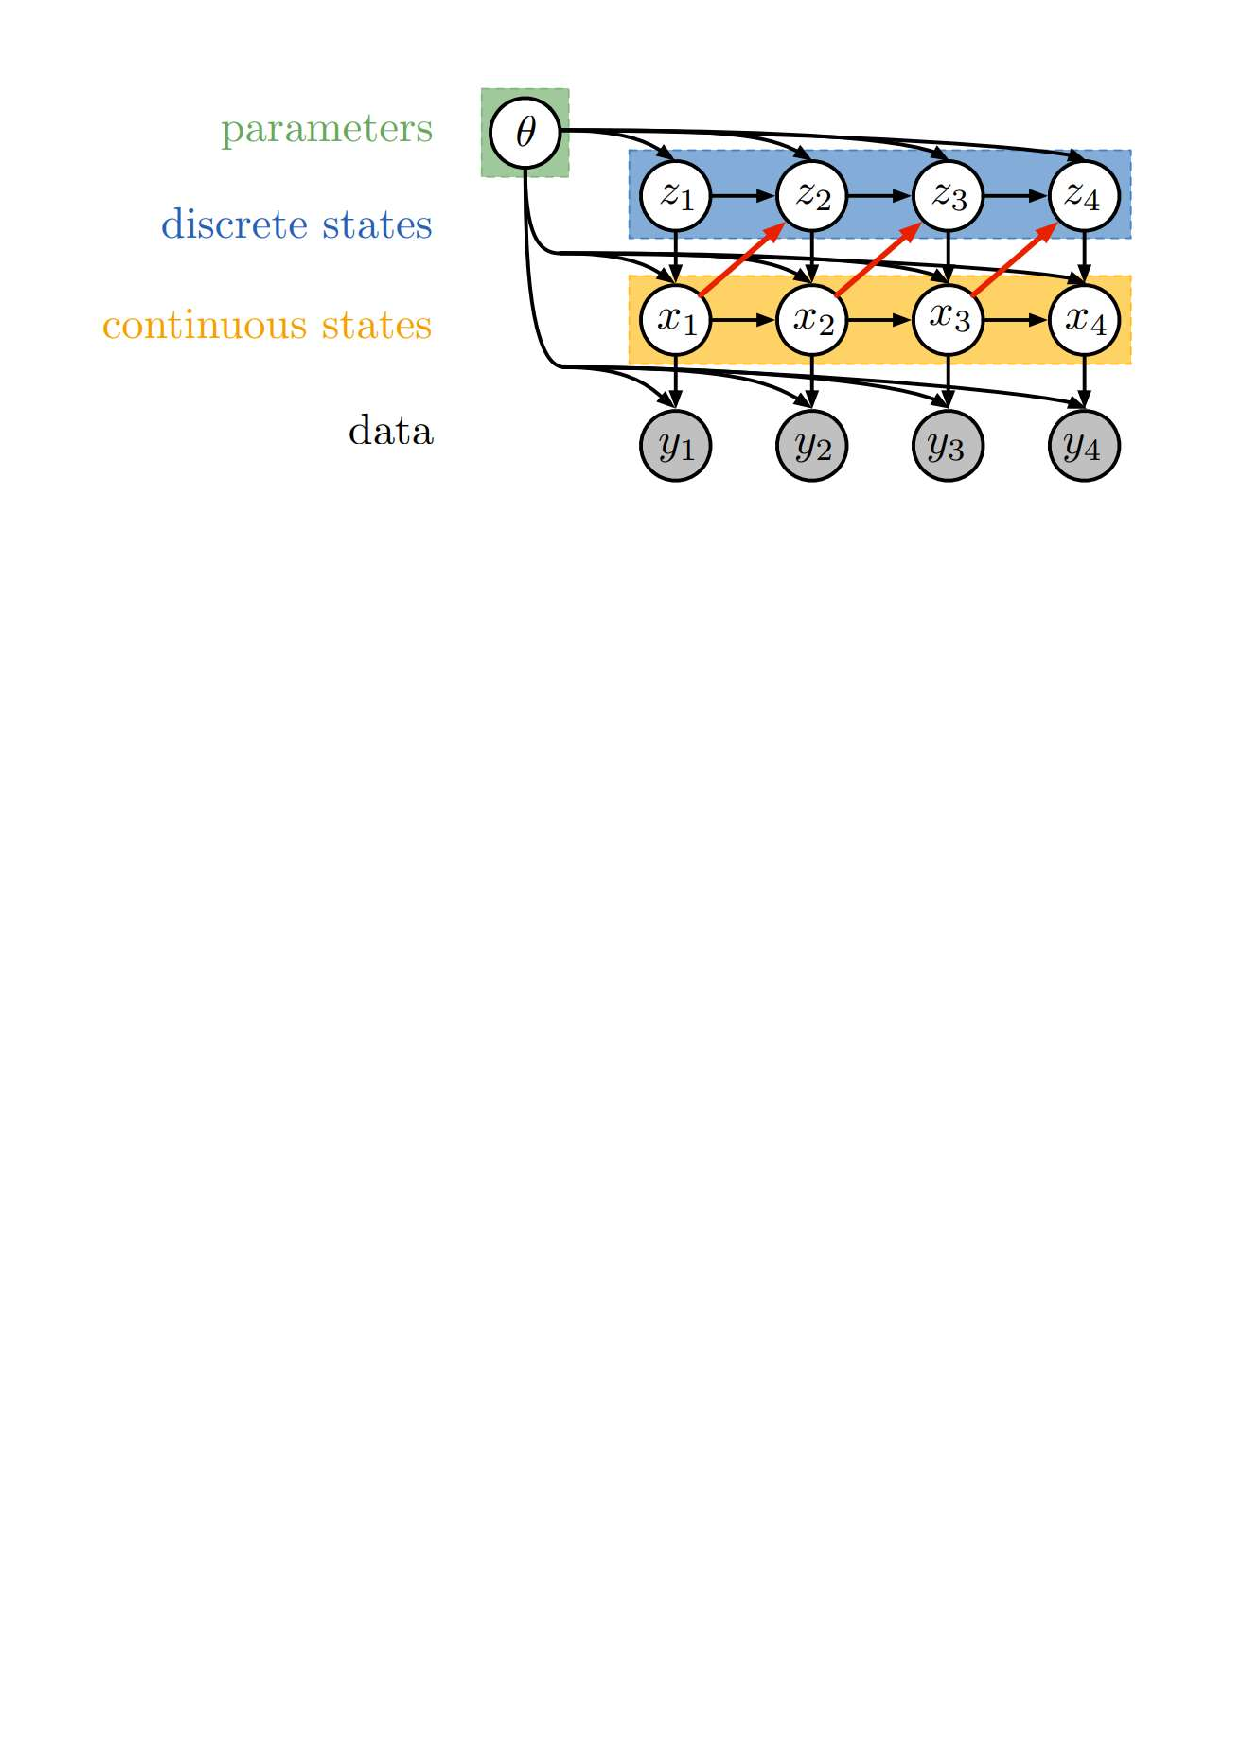
\includegraphics[scale=0.3]{gallery/rSLDS.pdf}
%    \caption{Graphical Model for the rSLDS}
%    \label{rLSDS}
%\end{figure}

    \end{frame}

\begin{frame}{Model}{Stick Breaking Logitstic Regression}
       \begin{tcolorbox}[colback=blue!10!white,colframe=blue!50!black,title=Stick Breaking Logitstic Regression,boxrule=2pt, boxsep=0.1em, left=0.1em, right=0.1em,
fontupper=\fontsize{8}{10}\selectfont] %,height=2in
\begin{enumerate}[\textbullet]
\item
\item 
    \item 
        \begin{itemize}
            \item 
            \item
        \end{itemize}
\end{enumerate}
\end{tcolorbox}

    \end{frame}

\begin{frame}{Model}{Inference}
        Daran

    \end{frame}


\section{Conclusion}

\begin{frame}{Frame Title}{Frame Subtitle}
        Rohin

    \end{frame}

\section{Next Step}

\begin{frame}{Frame Title}{Frame Subtitle}
        Rohin

    \end{frame}

\subsection{A Subsection}

    \begin{frame}{Frame Title}{Frame Subtitle}
        This is a frame with a title and a subtitle.

    \end{frame}

    \begin{frame}{\null}
        This is a frame with no title.
    \end{frame}

    \begin{frame}
        This is a frame with no header.
    \end{frame}

\subsection{Another Subsection}

    \begin{frame}{Text}
        \underline{This is underlined text.}

        \textit{This is italic text.}

        \textbf{This is bold text.}

        \texttt{This is mono-spaced text.}
    \end{frame}

    \begin{frame}{Lists}
        This is a bulleted list:
        \begin{itemize}
            \item An item

            \item Another item
            \begin{itemize}
                \item A subitem

                \item Another subitem
            \end{itemize}
        \end{itemize}

        This is a numbered list:
        \begin{enumerate}
            \item An item

            \item Another item
            \begin{enumerate}
                \item A subitem

                \item Another subitem
            \end{enumerate}
        \end{enumerate}
    \end{frame}

    \begin{frame}{Colored Blocks}
        \begin{block}{Block Title}
            This is a block.
        \end{block}

        \begin{alertblock}{Alert Block Title}
            This is an alertblock.
        \end{alertblock}

        \begin{example}
            This is an example block.
        \end{example}
    \end{frame}


%~~~~~~~~~~~~~~~~~~~~~~~~~~~~~~~~~~~~~~~~~~~~~~~~~%


\section{Second Section}

    \begin{frame}{Frame Title}
        This is a frame the second section.
    \end{frame}

    \begin{frame}{Frame Title}
        This is a frame with a...

        \pause

        \texttt{\textbackslash pause}.
    \end{frame}

\section{Bibliography}

    \nocite{einstein, knuthwebsite, latexcompanion}
    
    \begin{frame}{Bibliography}
        \bibliographystyle{plain}
        \bibliography{bibliography_file}
    \end{frame}

\end{document}
